\chapter{Bayesian Optimization}
Whereas traditional regression workflow is the following: From data, fit model parameters, make predictions using the parameters. 
The Bayesian framework allows us to skip the dependency of a single set of parameters and instead use all sets of parameters 
by treating the set of parameters as a random quantity, $\theta$. What is of interest is the predictive posterior distribution,  
\begin{align}\label{Predictive2}
    p(y|x, \mathcal{D})
\end{align}
% Before bringing the parameters/unknown quantities into play, we can ask: What quantities can we play
% with? This question is answered in two different ways in Gaussian process regression and Bayesian
% Neural network regression.

Bayesian optimization is essentially two steps: First, a probabilistic surrogate-model is fitted
to the available data $\mathcal{D}$ giving the predictive distribution \eqref{Predictive2}. Second,
the next sample point is chosen according to a so-called acquisition function, which in a sense
balance out the well-known concept, exploitation and exploration. Where exploitation will be chooing
the next point according to its expected improvement and exploration will be choosing the next point
in a region of high uncertainty and thereby help lower the overall uncertainty. We will first look at
the acquisition function used in this thesis, which is also the most commonly used: E   xpected improvement. 

\section{Acquisition function}
A popular choice of acquisition function is expected improvement, 
$$EI(x) = \mathbb{E}_{p(y|x,\mathcal{D})}[\max(0, y_{\min}-y)]$$
this will only look at the expectation of the values $y$, which improves the current best value.

\begin{figure}[H]
    \centering
    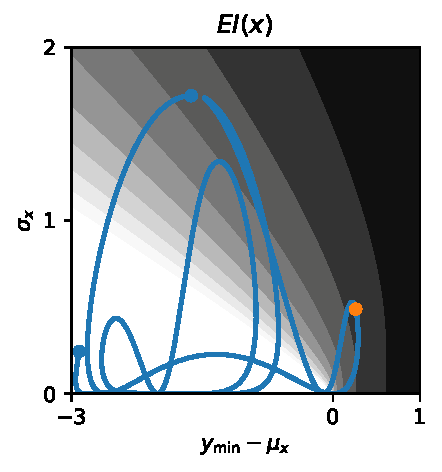
\includegraphics[width=0.8\textwidth]{Pictures/expected_improvement_illustration.pdf}
\end{figure}

In the following deveration
we assume the predictive distribution can be approxiamted by a normal distribution dependent on
the point of interest $x$ and the data $\mathcal{D}$ (note for the GP
it is in fact not an approximation), 
$$p(y|x,\mathcal{D}) \approx \mathcal{N}(y|\mu(x,\mathcal{D}), \sigma^2(x,\mathcal{D}))$$ where we
will change to a less clumpsy notation $\mathcal{N}(y|\mu_x,
\sigma^2_x):=\mathcal{N}(y|\mu(x,\mathcal{D}), \sigma^2(x,\mathcal{D}))$. This is completely fine
since we $x$ is fixed (and $\mathcal{D}$ is fixed) when evaluating the expected improvement in a point
$x$. %  $\sigma_x := \sigma^2(x,\mathcal{D})$ and $\mu_x := \mu(x,\mathcal{D})$
%as evaluated functions, i.e. numbers. 
Furthermore, the density of
a standard normal distribution is denoted $\phi(\cdot):=\mathcal{N}(\cdot | 0,1)$, and the cumlative
density function (CDF) of a standard normal distribution is denoted, $\Phi(\cdot) :=
\int_{-\infty}^{\cdot} \phi(\epsilon)d\epsilon$. We will now see that the normal approximation
of the predictive distribution yiels closed form solution to the expected improvement function, 

\begin{align*}
    E_{p(y|x,\mathcal{D})}[\max(0,y_{\min}-y)] &= \int \max(0,y_{\min}-y) p(y|x,\mathcal{D}) dy\\
    &\approx \int \max(0,y_{\min}-y) \mathcal{N}(y|\mu_x, \sigma_x^2) dy\\
    &= \int_{-\infty}^{y_{\min}} (y_{\min}-y) \frac{1}{\sigma_x}\phi\left(\frac{y-\mu_x}{\sigma_x}\right) dy\\
    &= \int_{-\infty}^{\frac{y_{\min}-\mu_x}{\sigma_x}} (y_{\min}-\mu_x-\sigma_x\epsilon) \frac{1}{\sigma_x}\phi\left(\epsilon\right) \sigma_x d\epsilon\\
    &= \int_{-\infty}^u \sigma_x \cdot (u-\epsilon) \phi(\epsilon) d\epsilon\\
    &=  \sigma_x \cdot \left( u\cdot \int_{-\infty}^u \phi(\epsilon) d\epsilon +\int_{-\infty}^u (-\epsilon)  \phi(\epsilon) d\epsilon \right) \\
    &= \sigma_x [u\Phi(u)+ \phi(u)]
\end{align*}

where $u:=\frac{y_{\min}-\mu_x}{\sigma_x}$. To understand the identity $\phi(u) = \int_{-\infty}^u
(-\epsilon)  \phi(\epsilon) d\epsilon$ used in the last equality, we first see that the antiderivative
is $\phi(\epsilon) = \frac{1}{\sqrt{2\pi}} \exp(\frac{-\epsilon^2}{2})$,
\begin{align*}
    \frac{d}{d \epsilon} \phi(\epsilon) &=  \frac{1}{\sqrt{2\pi}}\frac{d}{d \epsilon} \exp(\frac{-\epsilon^2}{2})\\
    &=  \frac{1}{\sqrt{2\pi}}\exp(\frac{-\epsilon^2}{2})(-\epsilon)\\
    &= -\epsilon \phi(\epsilon)
\end{align*}
and evaluating the rieman integral is equivalent to evaluate the antiderivative in its boundaries, giving the 
solution, 
$$\int_{-\infty}^u
(-\epsilon)  \phi(\epsilon) d\epsilon = \left[\phi(\epsilon)\right]_{-\infty}^u = \phi(u)-0 = \phi(u)$$ 

We can also explicily write the expected improvement as, 
$$EI(x) = (y_{\min}-\mu_x)\Phi\left(\frac{y_{\min}-\mu_x}{\sigma_x}\right)+ \sigma_x
\phi\left(\frac{y_{\min}-\mu_x}{\sigma_x}\right)]$$
where the first part can be interpretted as exploitation (favouring points with a large improvement $I(x) := (y_{\min}-\mu_x)$)
and the second part can be seen a exploitation (favouring points with high uncertainty.)
taking the derivative with respect to $I(x) := (y_{\min}-\mu_x)$ and $\sigma_x$, we see that expected improvement is 
is increasing if the improvement grows or if the variance $\sigma_x$ grows, i.e
$$\frac{\partial EI(x)}{\partial I(x)} = \Phi\left(\frac{y_{\min}-\mu_x}{\sigma_x}\right) > 0, \hspace*{0.5cm} 
\frac{\partial EI(x)}{\partial \sigma_x} = \phi\left(\frac{y_{\min}-\mu_x}{\sigma_x}\right) >0$$ 
<obs mistake in the book!!!?>





\begin{align*}
    \mathbb{E}_{y_*|\textbf{x}_*,D_n}[\max(0,y_{\min}-y_*)] &= ??\\
    \mathbb{E}[\min(0,y_{\min}-y_*)|\textbf{x}_*,D_n] &= \int_{-\infty}^\infty \min(0,y_{\min}-y_*) p(y_*|\textbf{x}_*,D_n) dy_*\\
    &= \int_{-\infty}^{y_{\min}} (y_{\min}-y_*) p(y_*|\textbf{x}_*,D_n) dy_*\\
    &\approx \frac{1}{N} \sum_{\theta \in \Omega } [y_{\min}-f_\theta(x)]
\end{align*}

where $\Omega = \{\theta|f_{\theta}(x)< y_{\min}\}$

%\section{uncertainties}
%Alatoric vs epistemic uncertainties 


\section{surrogate model}

\subsection{Discriminative model as surrogate model}
When talking about a probabilistic surrogate model we are always implicit talking about a
discriminative model: A model of the conditional distribution of the observation, $y$, 
conditional on $x$, i.e., 
$$p(y|x)$$
we also refer to this as the predictive distribution. Gaussian processes and Bayesian neural networks
are both discriminative models. There is no distribution over the input $x$, it is just given. 
This is indeed sufficient for a surrogate model, where we are interested in the predictive distribution. 

\subsection{Using a generative model as surrogate model}

Given a generative model over $x$ and $y$ paramitised with $\theta$, we are dealing with the joint distribution
$$p(x,y|\theta)$$
and we are interested in the condtional distribution of y given x, 
$$p(y|x, \theta_{y|x})$$
where we have put subscript on $\theta$ in order to jump up a level of abstraction since, 
in fact there is just a mapping between them $\theta_{y|x} := g(\theta, y, x)$ 

% $$\alpha p(y|x) + (1-\alpha) \mathcal{N}(0,1)$$

% so what should $\alpha$ be? Here we can find inspiration from a Poission point process. 


\begin{align*}
    p(y|x, \mathcal{D}) &= \int p(y|x,\theta_{y|x})p(\theta_{y|x}|\mathcal{D}) d\theta_{y|x}  \\
    &=  p(y|x,\hat \theta_{y|x})
\end{align*}
Where the last equation holds as we assume that $p(\theta_{y|x}|\mathcal{D})$ is a delta function
i.e. a point estimate with value $\hat \theta_{y|x}$. In the case of our Gaussian mixture model, 
we obtain a point estiamte from the EM algorithm for the variance $\Sigma_{y|k}$, mean value $\mu_{y|k}$ and proportion $\pi_{y|k}$
for each component $k = 1,2, \dots, K$
$$\hat \theta_{y|x} = (\hat\Sigma_{y|k}, \hat\mu_{y|k}, \hat\pi_{y|k})_{k=1}^K$$

However, we are not satisfied with the variance estimate for the regression, as it is way too small for areas with
no observed data. It is therefore necessary to manipulate the variance estimate accoring to that observation. 
We multiply the variance obtained using expectation-maximization on the joint distribution with the
inverse of the probability of the data $x$, and control that the scaling factor is not going wild!

$$\hat\Sigma_{y|k} =\Sigma_{y|k}^{GMM} \frac{1}{\max(p(x), 0.01)}$$

In a way, this is a manipulation in a Bayesian spirit, as we let prior and subjective knowledge influence the
varience prediction. 

\subsection{Inclusion of prior distribution}
The conditional distribution $p(y|x)$ is without a prior. Therefore
its beliefs is not really ok.. In the flavour of a Poission point process, 
we introduce the prior.. 
$$p_{bayes}(y|x) = \frac{p(x)\cdot N \cdot p(y|x) + \lambda p_{prior}(y)}{Z}$$
where the normalization constant $Z$ makes sure the manipulated density integrates
to 1, i.e. 
$$Z =\int p(x)\cdot N \cdot p(y|x) + \lambda p_{prior}(y) dy =p(x)\cdot N+\lambda $$


\begin{figure}[H]
    \centering
    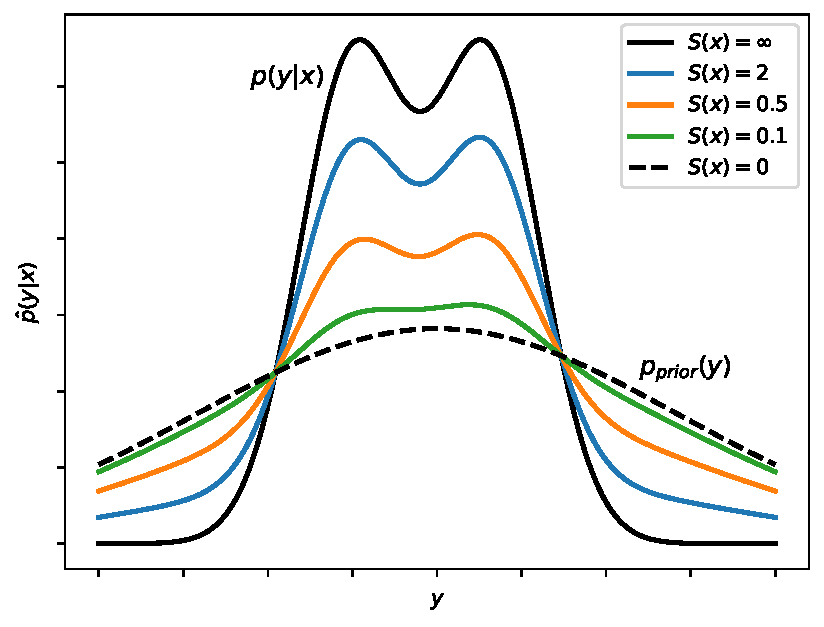
\includegraphics[width=0.5\textwidth]{Pictures/mixture_predictive_bayesian.pdf}
\end{figure}

\begin{figure}[H]
    \centering
    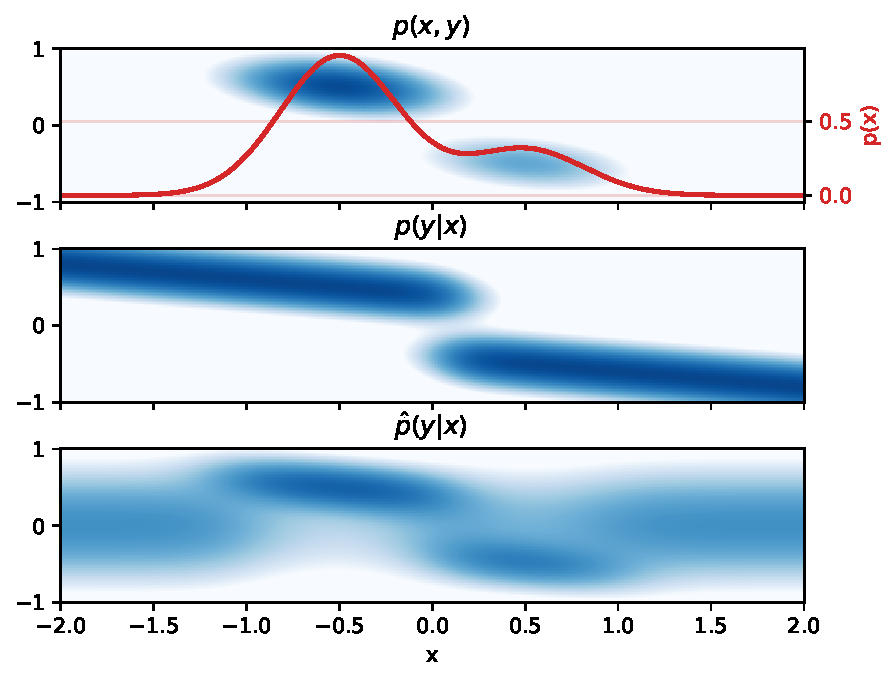
\includegraphics[width=0.5\textwidth]{Pictures/mixture_predictive_bayesian2D.pdf}
\end{figure}

\subsubsection*{mean of $p_{bayes}(y|x)$}
\begin{align*}
    E_{p_{bayes}(y|x)}[y] &= \int y \cdot \frac{f(n,p(x)) \cdot p(y|x) + \lambda p_{prior}(y)}{Z} dy\\
    &= \left(p(x)\cdot N \cdot E_{p(y|x)}[y] + \lambda \cdot E_{p_{prior}(y)}[y] \right) \frac{1}{Z}\\
    &= \frac{p(x)\cdot N\cdot E_{p(y|x)}[y]}{p(x)\cdot N+\lambda}
\end{align*}

\subsubsection*{variance of $p_{bayes}(y|x)$}
We first calculate the second moment, 
\begin{align*}
    E_{p_{bayes}(y|x)}[y^2] &= \int y^2 \cdot \frac{p(x)\cdot N \cdot p(y|x) + \lambda p_{prior}(y)}{Z} dy\\
    &= (p(x)\cdot N\cdot E_{p(y|x)}[y^2] + \lambda E_{p_{prior}(y)}[y^2] ) \frac{1}{Z}\\
    &= \frac{p(x)\cdot N \cdot(Var_{p(y|x)}[y]+E_{p(y|x)}[y]^2) + \lambda Var_{p_{prior}(y)}[y]}{p(x)\cdot N+\lambda}
\end{align*}

So the variance is calculated as, 
$$V_{p_{bayes}(y|x)}[y] = E_{p_{bayes}(y|x)}[y^2] - E_{p(x,y)}[y]^2$$

\subsubsection*{implementation}
It is not necessary to calculate the conditional distribution, since, using Bayes rule
$$p(y|x) = \frac{p(x,y)}{p(x)}$$
so gives
$$p_{bayes}(y|x) = \frac{p(x)\cdot N \cdot p(y|x) + \lambda p_{prior}(y)}{Z} = \frac{N \cdot p(x,y) + \lambda p_{prior}(y)}{Z}$$

$$E_{p(x,y)}[y] = \int_y \int_x yp(x,y) dx dy = \int_y y p(y) dy = E_{p(y)}[y]$$